\documentclass[12pt,spanish]{article}
% aprovechamiento de la p\'agina -- fill an A4 (210mm x 297mm) page
% Note: 1 inch = 25.4 mm = 72.27 pt
% 1 pt = 3.5 mm (approx)

% vertical page layout -- one inch margin top and bottom
\topmargin      -10 mm   % top margin less 1 inch
\headheight       0 mm   % height of box containing the head
\headsep          0 mm   % space between the head and the body of the page
\textheight     255 mm   % the height of text on the page
\footskip         7 mm   % distance from bottom of body to bottom of foot

% horizontal page layout -- one inch margin each side
\oddsidemargin    0 mm     % inner margin less one inch on odd pages
\evensidemargin   0 mm     % inner margin less one inch on even pages
\textwidth      159 mm     % normal width of text on page

\setlength{\parindent}{0pt}

\usepackage{tikz}
\usetikzlibrary{automata,positioning}

\usepackage[doument]{ragged2e}
\usepackage{babel}
\usepackage[utf8]{inputenc}
\usepackage{amsmath,amsthm,mathtools}
\usepackage{amsfonts,amssymb,latexsym}
\usepackage{enumerate}
\usepackage{subfigure, float, graphicx, caption}
\captionsetup[table]{labelformat=empty}
\captionsetup[figure]{labelformat=empty}
\definecolor{RojoAnayelRey}{rgb}{1,.25,.25}
\usepackage[bookmarks=true,
            bookmarksnumbered=false, % true means bookmarks in 
                                     % left window are numbered                         
            bookmarksopen=false,     % true means only level 1
                                     % are displayed.
            colorlinks=true,
            linkcolor=webred]{hyperref}
\definecolor{webgreen}{rgb}{0, 0.5, 0} % less intense green
\definecolor{webblue}{rgb}{0, 0, 0.5}  % less intense blue
\definecolor{webred}{rgb}{0.5, 0, 0}   % less intense red
\definecolor{dkgreen}{rgb}{0,0.6,0}
\definecolor{gray}{rgb}{0.5,0.5,0.5}
\definecolor{mauve}{rgb}{0.58,0,0.82}
\definecolor{MistyRose}{RGB}{255,228,225}
\definecolor{LightCyan}{RGB}{224,255,255}

% \usepackage{beton}
% \usepackage[T1]{fontenc}

% Theorem environments

%% \theoremstyle{plain} %% This is the default
\newtheorem{theorem}{Teorema}[section]
\newtheorem{corollary}[theorem]{Corolario}
\newtheorem{lemma}[theorem]{Lema}
\newtheorem{proposition}[theorem]{Proposici\'on}
%\newtheorem{ax}{Axioma}

\theoremstyle{definition}
\newtheorem{definition}{Definici\'on}[section]
\newtheorem{algorithm}{\textrm{\bf Algoritmo}}[section]

\theoremstyle{remark}
\newtheorem{remark}{Observaci\'on}[section]
\newtheorem{example}{Ejemplo}[section]
\newtheorem{exercise}{Ejercicio}%[section]
%\newenvironment{solution}{\begin{proof}[Solution]}{\end{proof}}
\newenvironment{solution}{\begin{proof}[Solución]}{\end{proof}}
\newtheorem*{notation}{Notaci\'on}

%\numberwithin{equation}{section}

%\newcommand{\regla}[2]{
%\begin{array}{c}
%#1\\
%\hline
%#2\\
%\end{array}
%}
\begin{document}

\title{Modelos de Computación: \\ Relación de problemas 1}
\author{David Cabezas Berrido}
\date{\vspace{-5mm}}
\maketitle

\setcounter{exercise}{16}
\begin{exercise}~ Autómata finito determinista que reconoce el
  lenguaje
  \[L_1=\{u\in\{0,1\}^* \ | \text{ el número de 1's no es múltiplo de 3}\}\] \vspace{-10mm}
  \begin{figure}[H]
  \centering
  \subfigure{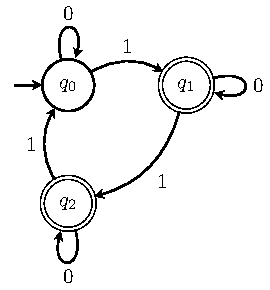
\includegraphics[width=60mm]{17_1}}
\end{figure}
\vspace{-10mm}
  \[L_2=\{u\in\{0,1\}^* \ |\text{ el número de 0's es par}\}\] \vspace{-10mm}
  \begin{figure}[H]
  \centering
  \subfigure{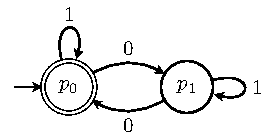
\includegraphics[width=70mm]{17_2}}
  \end{figure} \vspace{-5mm}
  Ahora sólo tenemos que intersecar los dos autómatas para formar el
  deseado, el que reconoce el lenguaje
  \[L_3=\{u\in\{0,1\}^* \ |\text{ el número de 1's no es múltiplo de 3 y el número de 0's es par}\}\]
  \begin{figure}[H]
  \centering
  \subfigure{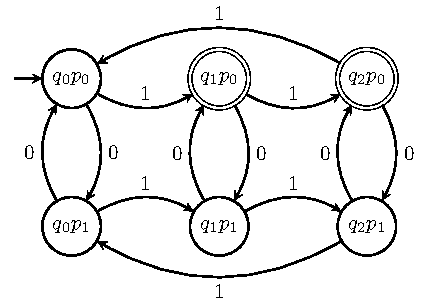
\includegraphics[width=75mm]{17_3}}
  \end{figure}
  
\end{exercise}

\setcounter{exercise}{21}
\begin{exercise}~ Para hallar la expresión regular que representa el lenguaje aceptado por el autómata \vspace{-5mm}
\begin{figure}[H]
  \centering
  \subfigure{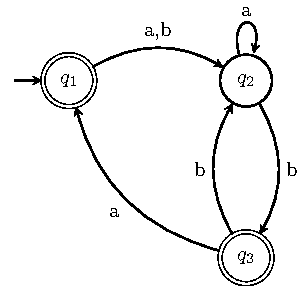
\includegraphics[width=50mm]{22}}
\end{figure} \vspace{-5mm}
usaremos el algoritmo visto en clase (sólo mostraré un par de iteraciones)
\begin{align*}
  r_{11}^3&+r_{13}^3 \\
  r_{11}^2+r_{13}^2(r_{33}^2)^*r_{31}^2&+r_{13}^2+r_{13}^2(r_{33}^2)^*r_{33}^2 \\
  \varepsilon+(a+b)a^*b(a(a+b)a^*b)^*a&+(a+b)a^*b(a(a+b)a^*b)^* \\
  \varepsilon+(a+b)a^*b(a(a&+b)a^*b)^*(a+\varepsilon)
\end{align*}
\end{exercise}

\begin{exercise}~ Para probar que
  $B_n=\{a^k \ | \text{ k es múltiplo de n}\}=\{a^{kn} \ | \ k \in
  \mathbb{N}\}$ es regular para todo $n$, construiremos un autómata
  finito determinista que lo reconozca.

  $B_0=\{\varepsilon\}$ es trivialmente regular, lo reconoce el autómata \vspace{-5mm}
\begin{figure}[H]
  \centering
  \subfigure{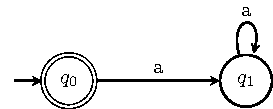
\includegraphics[width=50mm]{23_b0}}
\end{figure} \vspace{-5mm}
$B_1=\{a\}^*$ es reconocido por \vspace{-7mm}
\begin{figure}[H]
  \centering
  \subfigure{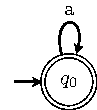
\includegraphics[width=20mm]{23_b1}}
\end{figure}
$B_2=$ palabras sobre $\{a\}^*$ con número par de $a$'s es reconocido por
\begin{figure}[H]
  \centering
  \subfigure{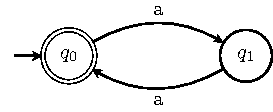
\includegraphics[width=50mm]{23_b2}}
\end{figure}

$B_3$ por 
\begin{figure}[H]
  \centering
  \subfigure{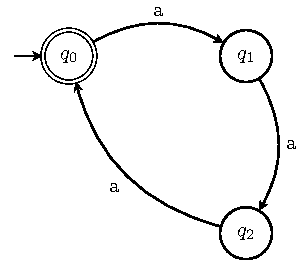
\includegraphics[width=50mm]{23_b3}}
\end{figure}

De esta forma,
$M_n=(\{q_0,\ldots,q_{n-1}\},\{a\},q_0,\delta_n,\{q_0\})$ con
\\ $\delta_n(q_i,a)=q_{(i+1)\%n}$ $\forall i=0,\ldots,n-1$ es un
autómata finito determinista que reconoce el lenguaje $B_n$
$\forall n\geq 2$. \\

También puede razonarse que $B_n=(a_1a_2\ldots a_n)*$ donde
$a_i=a \ \forall i$.
\end{exercise}

\begin{exercise}~ Dado un lenguaje regular $L$, probaremos que los
  siguientes lenguajes son regulares \\
  
  $a) NOPREFIJO(L)=\{u\in L \ |$ ningún prefijo propio de $u$ pertenece a $L\}$ \\

  Buscamos eliminar las palabras del lenguaje que tienen prefijos
  propios que pertenecen al lenguaje, podemos conseguir esto con tan
  sólo hacer inaccesibles algunos de los estados finales del autómata.

  Supongamos que $M=(Q,A,q_0,\delta,F)$ es un autómata finito
  determinista que reconoce a $L$. Construimos
  $M'=(Q\cup\{p\},A,q_0,\delta',F)$ y definimos $\delta'$ de la
  siguiente forma
  \begin{align*}
    \delta'(f,a)=&p \quad \forall f \in F, \ \forall a \in A \\
    \delta'(p,a)=&p \quad \forall a \in A \\
    \delta'(q,a)=&\delta(q,a) \quad \text{en el resto de casos}
  \end{align*}
  Si $u$ es aceptada por $M'$, significa que $\delta'(q_0,u) \in F$,
  además no hemos pasado por ningún estado final en medio (de haberlo
  hecho acabaría ciclando en $p$), por lo que siempre hemos aplicado
  la definición del resto de casos, esto significa que ningún prefijo
  propio de $u$ es aceptado por $M'$ y que todas las palabras
aceptadas por $M'$ son de $L$. \\

  Resumiendo, hemos encontrado un autómata finito determinista que
reconoce $NOPREFIJO(L)$, luego es regular. \\

  $b) NOEXTENSION(L)=\{u\in L \ | \ u$ no es prefijo propio de ninguna
palabra de $L\}$ \\

  Si un estado es final pero leyendo más símbolos se puede llegar a
otro (o el mismo) estado final, se deben eliminar del lenguaje las
palabras que lleven a ese estado. Esto lo conseguimos eliminando
estados finales.

  Supongamos que $M=(Q,A,q_0,\delta,F)$ es un autómata finito
determinista que reconoce a $L$. Construimos $M'=(Q,A,q_0,\delta,F')$
donde
  \[F'=\{q\in F \ | \ \nexists u \in A^*, \ \nexists f \in F :
(q,u)\vdash^* (f,\varepsilon)\}\]

De esta forma, $M'$ sólo acepta palabra de $L$. Además, de toda
palabra $u$ aceptada por $M'$, sabemos que no existe otra palabra $v
\neq \varepsilon$ tal que $uv \in L$ justo como queríamos. \\

  Resumiendo, hemos encontrado un autómata finito determinista que
reconoce $NOEXTENSION(L)$, luego es regular. \\
\end{exercise}

\end{document}
